\section{Experiments}
\label{sec:exp}

The purpose of this experiment is to check how our generalized critic performs by comparison to a regular critic on top of a common actor, while paying a particular attention to the following factors:
\begin{enumerate}
\item the tested environments, and how differently they react to the implemented method;
\item the hyperparameters of the advantage, specifically the $\lambda$ coefficient;
\item the aggregation function, and how its parameters affect the average return.
\end{enumerate}

We will then provide the average total reward for each set of experiments and an interpretation of the results.

\subsection{Experiment Setting}
% In the case of a continuous action space, $\pi$ is a gaussian distribution. <- add this to experiments
For the sake of this experiment, we will use continuous control tasks from the OpenAI Gym \cite{brockman2016openai} toolkit collection. In particular, we use the variants that are based on the Bullet physics engine from the Pybullet package: AntBulletEnv-v0, Walker2DBulletEnv-v0 and HumanoidBulletEnv-v0. Those environments are simulated with the Bullet physics engine, and are a free alternative to the environments that use the commercial MuJoCo physics engine \cite{todorov2012mujoco}. 

The experiment setting is as follows: for every run, we implement a generalized critic with two values for the advantage function based on the same estimate of $V(s_t)$ by calculating a GAE function with different values for the $\lambda$ coefficient. The aggregation function in this case is defined as a convex combination, with a weight vector $\beta$. The final critic value is given as follows

\[ \mathcal{F}(\hat{A}_1^{GAE(\gamma, \lambda_1)}, \hat{A}_2^{GAE(\gamma, \lambda_2)}) = \beta_1\hat{A}_1^{GAE(\gamma, \lambda_1)}+\beta_2\hat{A}_2^{GAE(\gamma, \lambda_2)} \]

such that $\beta_1 + \beta_2 = 1$.

We conduct two sets of experiments: 
\begin{enumerate}
\item To observe the effect of the critic on each of the environments, we set $\beta=(0.5, 0.5)$ and experiment with three generalized critics with their vectors of $\lambda$ values corresponding to (0.97, 0.93), (0.97, 0.99) and (0.99, 0.97) respectively. (results reported in table \ref{tab:reslam}
\item For one of the previous generalized critics ($\lambda$ = (0.97, 0.93)), we test three different aggregation function such that $\beta_1 = (0.5, 0.5)$, $\beta_2 = (0.75, 0.25)$ and $\beta_3 = (0.25, 0.75)$ (results in figure \ref{fig:res})
\end{enumerate}

The policy optimization method that we use for this experiment is a Proximal Policy Optimization\cite{schulman2017proximal} with the clip variant. The policy update is performed as follows:

\begin{align*}
\theta_{k+1} = & \arg \max_{\theta} \frac{1}{| \mathcal{D}_k | T} \sum_{\tau \in \mathcal{D}_k} \sum_{t=0}^T \\ 
& \min \left(\frac{\pi_{\theta}(a_t\bar s_t)}{\pi_{\theta_k}(a_t\bar s_t)} A^{\pi_{\theta_k}}(a_t, s_t), g(\epsilon, A^{\pi_{\theta_k}}(a_t, s_t))\right)
\end{align*}

\subsection{Experiment Results}

Table \ref{tab:reslam} shows the average returns over 5 random seeds for each generalized critic variant after two million timesteps. The results are rounded to the second decimal.

\begin{table}[!htb]
\begin{tabular}{p{22mm}p{14mm}p{15mm}p{11mm}}
Algorithm & Walker2D & Humanoid & Ant\\
PPO ($\lambda$ = 0.97) & - & - & - \\
\hline
$\lambda$ = (0.97, 0.93) & 718,80 & 1535,21 & 108,23  \\ 
\hline
$\lambda$ = (0.97, 0.99)& 688,64 & 1218,36 & 105,31  \\ 
\hline
$\lambda$ = (0.99, 0.97)& 752 & 1080,83 & 106,99 \\ 
\end{tabular}
\caption{Performance for three generalized critics across environments}
\label{tab:reslam}
\end{table}



% Below is an example of how to insert images. Delete the ``\vspace'' line,
% uncomment the preceding line ``\centerline...'' and replace ``imageX.ps''
% with a suitable PostScript file name.
% -------------------------------------------------------------------------
\begin{figure}[!htb]

\begin{minipage}[b]{.48\linewidth}
  \centering
  \centerline{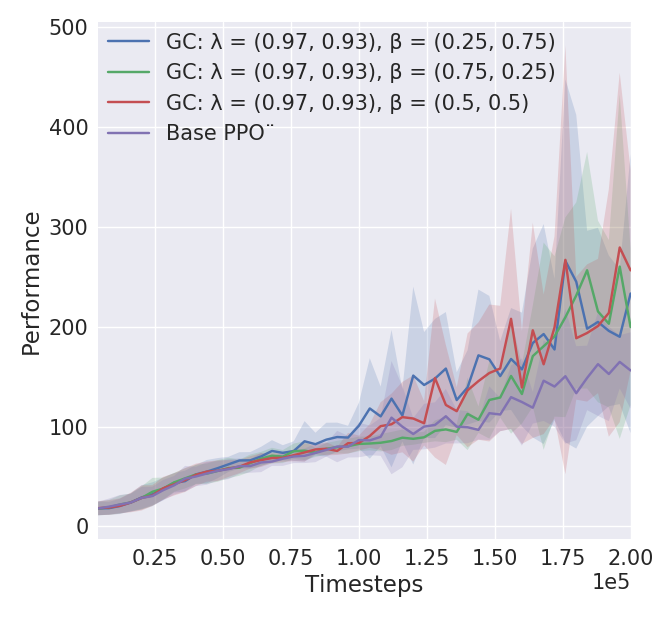
\includegraphics[width=4.0cm]{images/WalkerCoef}}
%  \vspace{2.0cm}
  \centerline{(a) Walker2DBulletEnv-v0}\medskip
\end{minipage}
\begin{minipage}[b]{.48\linewidth}
  \centering
  \centerline{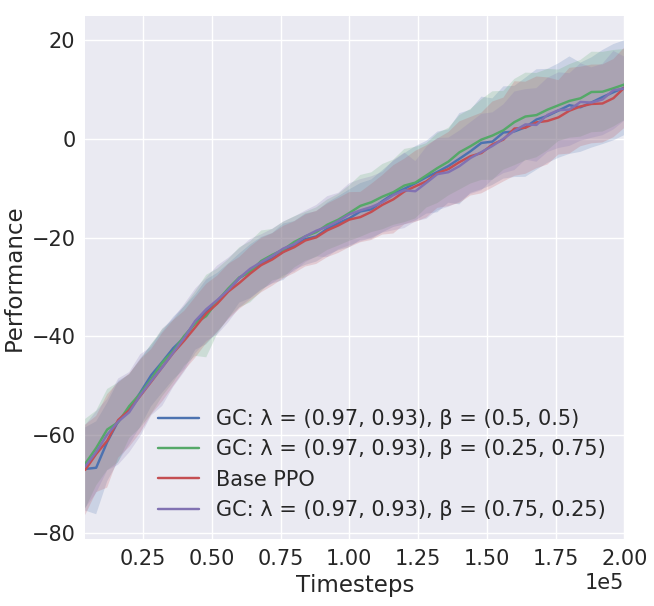
\includegraphics[width=4.0cm]{images/HumanoidCoef}}
%  \vspace{2.0cm}
  \centerline{(b) HumanoidBulletEnv-v0}\medskip
\end{minipage}

%
\begin{minipage}[b]{\linewidth}
  \centering
  \centerline{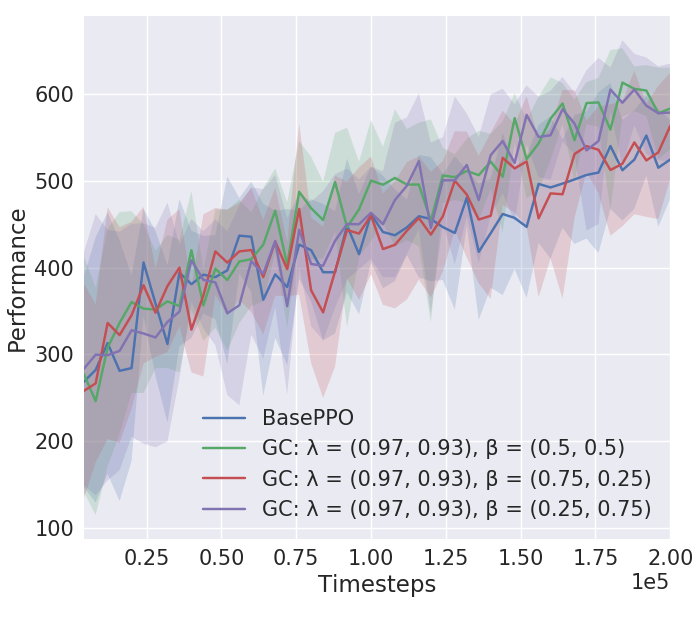
\includegraphics[width=4.0cm]{images/AntCoef}}
%  \vspace{1.5cm}
  \centerline{(c) AntBulletEnv-v0}\medskip
\end{minipage}
%\hfill
%\begin{minipage}[b]{0.48\linewidth}
%  \centering
%  \centerline{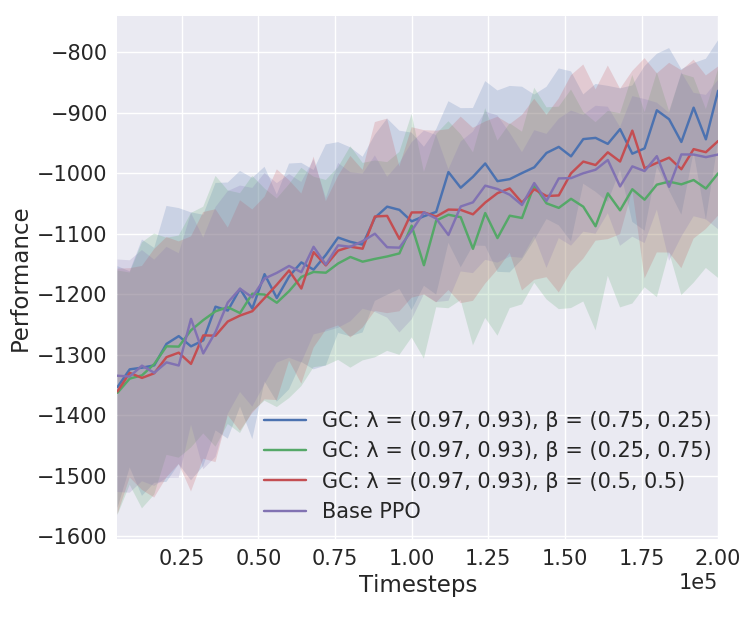
\includegraphics[width=4.0cm]{images/PendulumCoef}}
%  \vspace{1.5cm}
%  \centerline{(d) Pendulum}\medskip
%\end{minipage}
%
\caption{Performance of different coefficients for the aggregation function across environments.}
\label{fig:res}
%
\end{figure}


% To start a new column (but not a new page) and help balance the last-page
% column length use \vfill\pagebreak.
% -------------------------------------------------------------------------
%\vfill
%\pagebreak

